\chapter[Introdução]{Introdução}
\label{sec:introduction}

\section{Motivação}
A fluido-dinâmica tem grande valor acadêmico para estudantes nos cursos de graduação em engenharia, dada a extensa lista de aplicações industriais \cite{CFD_in_learing_2}. Exemplos são numerosos, como o estudo da combustão, aerodinâmica de veículos e aeronaves, climatologia, oceanografia, dentre outros.
Mas, haja vista a complexidade do tema, não é uma tarefa simples a compreensão dos conceitos mais abstratos que envolvem geometrias arbitrárias e fluxos turbulentos \cite{hasan}. Apesar disso, estas são partes essenciais do assunto, uma vez que se aproximam de casos práticos na indústria.

A mecânica dos fluidos permite o aumento na eficiência de processos mecânicos, como, por exemplo, no caso das máquinas térmicas. As transformações energéticas têm como subproduto energia térmica. Tirar essa energia do sistema de forma eficiente resulta em ganho de eficiência e aumento da longevidade dos equipamentos. Por isso, tem-se o estudo da mecânica dos fluidos como um dos grandes pilares da busca da indústria por eficiência energética e sustentabilidade.

A mecânica dos fluidos é um tópico muito estudado no meio acadêmico. A natureza não linear do fenômeno \cite{John} impossibilita soluções gerais analíticas. Consequentemente, na grande maioria dos casos, métodos numéricos tornam-se necessários para o entendimento dos fenômenos. Quando Simulações Numéricas Diretas (DNS) não são uma opção, aproximações devem ser feitas para que se viabilize a solução das equações de Navier-Stokes, como modelos de fechamento da turbulência, ajustes e aproximações. Para estes casos, discretizando-se o espaço e o tempo, resolver tais sistemas lineares requer enorme poder computacional, uma vez que o número de elementos necessários para simular adequadamente o fenômeno é muito grande. RANS, URANS e LES foram desenvolvidos como forma de otimizar a computação. Eles consistem em não resolver numericamente a equação de Navier-Stokes em todas as escalas necessárias, mas em vez disso substituir alguns tensores e outros termos não lineares por aproximações conceituais e experimentais, simplificando o cálculo.

Tais métodos são importantes porque oferecem uma solução de forma bem mais eficiente. A abordagem DNS (Simulação Numérica Direta) exige um alto trabalho computacional, pois considera todas as escalas de complexidade, nem mesmo sendo possível ou viável na maioria dos casos \cite{Kawamura}, como explicado no trabalho de H. Kawamura, H. Abe e Yuichi Matsuo \cite{Abe}. Mas, por outro lado, esses métodos aproximados resultam em imprecisões matemáticas.

O MFSim é uma ferramenta desenvolvida no Laboratório de Mecânica dos Fluidos pelo programa de pós-graduação da Faculdade de Engenharia Mecânica (FEMEC) da Universidade Federal de Uberlândia (UFU). Ele vem sendo desenvolvido de forma contínua a 12 anos e busca oferecer soluções computacionais a problemas de dinâmica dos fluidos de forma computacional, fazendo o uso dos métodos anteriormente citados. Neste trabalho, o software é utilizado em  uma análise comparativa entre seus resultados com os obtidos de forma semi analítica com a metodologia aqui descrita.

Dessa forma, no presente trabalho, os autores, a partir de métodos ativos de ensino \cite{CFD_in_learing}, desenvolvem um método semi-analítico para simular o escoamento em canais de Poiseuille \cite{Poiseuille} entre duas placas planas. Os resultados desse método são então comparados com resultados de ensaios em DNS e no programa de simulação fluidodinâmica MFSim.

\section{Perspectiva histórica}

O estudo da mecânica dos fluidos tem origem na relação do homem com a água, que sempre foi um recurso vital e determinante na sobrevivência dos povos. Começou formalmente com Archimedes que desenvolveu as leis da flutuação, que postulam que a força responsável por fazer um objeto flutuar é igual à massa do volume deslocada de dita substância \cite{dijksterhuis2014archimedes}. Em sequência tem-se a escola alexandrina onde se desenvolveram bombas hidráulicas sendo também estudadas diversas aplicações de escoamentos confinados, como o relógio de água de Ctesibius (Fig. \ref{image:ctesibius}).

\begin{figure}[htb]
	\begin{center}
    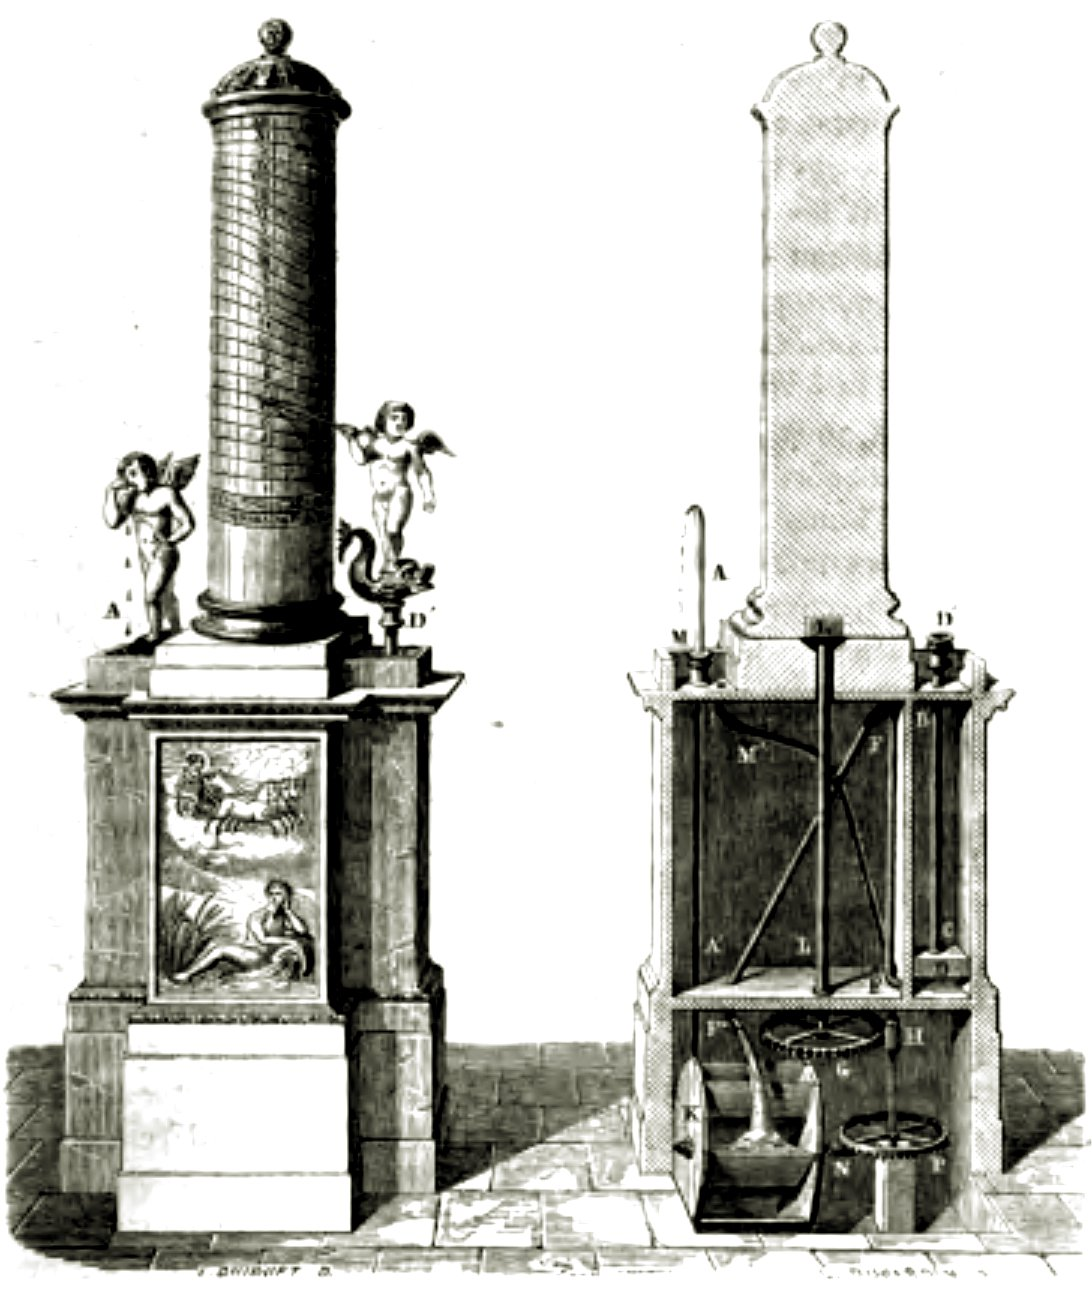
\includegraphics[scale=0.07]{ctesibius.jpeg}
	\end{center}
	\caption{\label{image:ctesibius} Relógio de água de Ctesibius, visualização criada pelo arquiteto francês Claude Perrault}
	\legend{Fonte: \citeonline[Fig. 16 et 17.]{argo}}
\end{figure}

Após isto, durante a idade média houveram os estudiosos islâmicos que desenvolveram pesquisas no campo da hidro-estática. Foi observada a diferença de peso entre água doce, salgada, quente e fria, calculando-se a massa específica das substâncias \cite{history_engeneering}. Então houveram grandes mestres como Benedetto Castelli, Evangelista Torricelli e Blaise Pascal que desenvolveram seus estudos formais sobre o tema e avançaram de forma significativa a compreensão sobre o comportamento da pressão e o movimento dos fluidos em uma série de experimentos bem documentados.

Houveram, então, os estudos de Isaac Newton, onde ele descreve fluidos incompressíveis e as forças viscosas que governam seu movimento a baixos números de Reynolds \cite{aristeu}. Em seus estudos ele descreve a relação que existe entre o esforço de cisalhamento e o gradiente de velocidade, definindo assim os chamados fluidos newtonianos:

\begin{equation}
    \tau = \mu \frac{d u}{d x}
\end{equation}

Além da viscosidade, Newton também estudou ondas e orifícios em reservatórios de água. Suas contribuições para o cálculo, conservação de energia e dinâmica de corpos rígidos também foram determinantes para os grandes pensadores que vieram depois.

Outro grande pensador foi Daniel Bernoulli. Ele estudou a transformação de energia da velocidade dos fluidos em pressão \cite{1570009750104671360}, relacionando a energia interna às diferenças de velocidade e energia potencial gravitacional:

\begin{equation}
    \frac{1}{2}\rho u^2 + P + \rho * g * h = ctt.
\end{equation}

Assim teve-se uma compreensão mais completa sobre o comportamento dos fluidos em escoamentos confinados.

Tais estudos acadêmicos culminaram com os estudos de  Claude-Louis Navier e George Gabriel Stokes, que desenvolveram as equações de Navier-Stokes, que, baseadas na conservação de energia conseguem descrever o movimento dos fluidos newtonianos:

\begin{equation}
\rho \vec{g}-\nabla \vec{p}+\eta \cdot \nabla^{2} \vec{u}=\rho \cdot\left(\vec{u} \cdot \nabla \vec{u}+\frac{\partial \vec{u}}{\partial t}\right)
\end{equation}

As formulações de Navier-Stokes são equação diferenciais parciais, cuja solução exata nunca foi encontrada para casos gerais. É possível, a partir de simplificações e ajustes, desconsiderar alguns termos de forma a se conseguir soluções exatas para casos suficientemente simples \cite{Cengel}. Mas a simplicidade desses casos os tornam pouco aplicáveis em problemas reais de engenharia.

Um exemplo de sistema simplificado é o escoamento de Poiseuille \cite{Poiseuille}. Nele, tem-se um escoamento Newtoniano e laminar entre duas placas planas infinitas de distância $h$. Para este caso, é possível se conseguir uma solução analítica para o perfil de velocidade que pode ser descrito pela equação que segue:

\begin{equation}
  u(y) = \frac{G}{2\mu}y (h - y).
\end{equation}

Onde G é um gradiente de pressão constante no sentido da corrente ($G = -\frac{dp}{dx}$), e $\mu$ é o coeficiente de viscosidade. Para casos não laminares, ou seja, em que o fluido se movimenta não só na direção e sentido do fluxo, essa equação já se distancia da realidade.
